
%(BEGIN_QUESTION)
% Copyright 2006, Tony R. Kuphaldt, released under the Creative Commons Attribution License (v 1.0)
% This means you may do almost anything with this work of mine, so long as you give me proper credit

Oppdriftsprinsippet kan brukes til å lage en nivåtransmitter som gir utgangssignal proporsjonalt med vektendringen til en ``fortrenger''-stav som henger i væske:

$$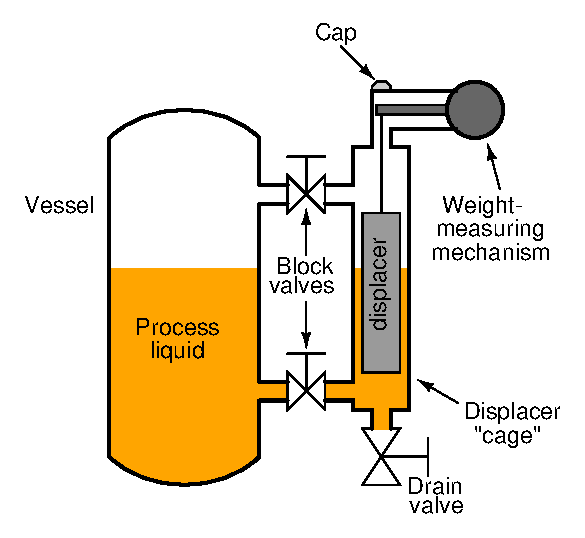
\includegraphics[width=15.5cm]{i00276x01.eps}$$

Ofte er fortrengeren montert i et eget ``cage'' for enkel uttak fra prosess, som vist over, eller montert direkte i prosesstanken slik:

$$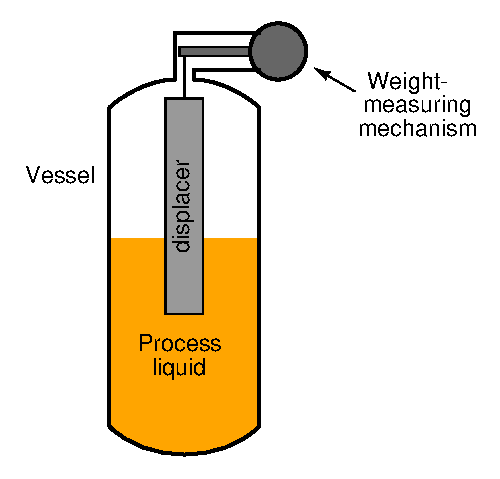
\includegraphics[width=15.5cm]{i00276x02.eps}$$

Hvis tanken er åpen og væsken er turbulent på grunn av miksing eller annen omrøring, fyller et \textit{stilling well} samme funksjon som et cage:

$$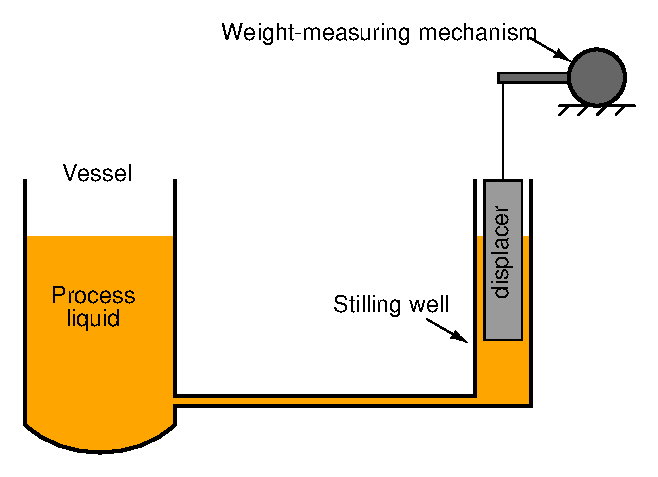
\includegraphics[width=15.5cm]{i00276x03.eps}$$

For å kalibrere et slikt instrument må det isoleres fra prosessvæsken.  Noen ganger betyr dette bare å stenge blokkventiler og tømme cage.  Andre ganger må fortrengermekanismen tas helt ut av tanken.  Men når fortrengeren henger tørt, oppstår problemet med å simulere 100\% tilstand for kalibrering.

Beskriv en måte å få fortrengeren til å ``tro'' den er helt neddykket i prosessvæske når den i virkeligheten henger fritt i luft.  Forklar hvordan du kan simulere denne tilstanden \textit{presist} og \textit{nøyaktig}, og tilsvarende enhver delvis neddykket tilstand.

\underbar{file i00276}
%(END_QUESTION)





%(BEGIN_ANSWER)

Én måte å simulere full tilstand på er å bruke en \textit{håndvekt}:

$$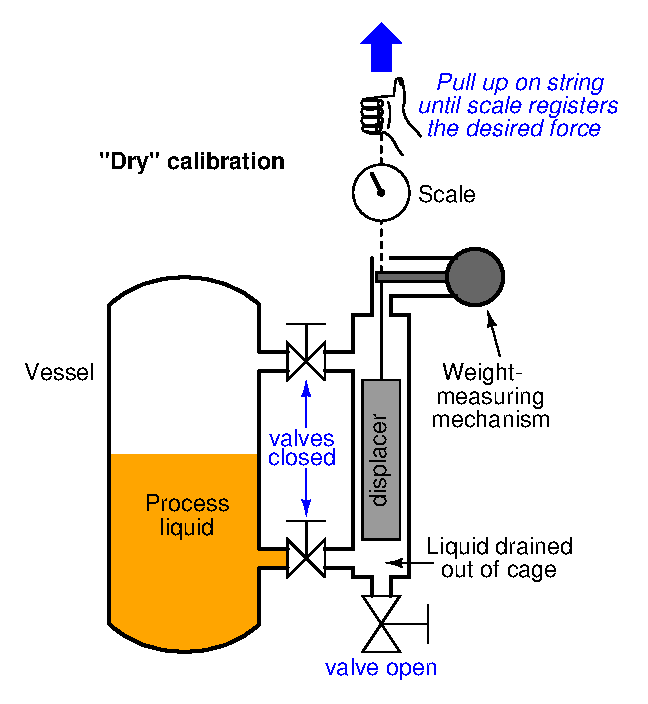
\includegraphics[width=15.5cm]{i00276x04.eps}$$

%(END_ANSWER)





%(BEGIN_NOTES)


%INDEX% Measurement, level: displacer (buoyancy)

%(END_NOTES)
